\documentclass{article}
\usepackage[T1]{fontenc}
\usepackage{lmodern}
\usepackage{graphicx}
\usepackage{amsmath,amssymb}
\usepackage[a4paper,margin=2cm]{geometry}
\usepackage[absolute,overlay]{textpos}
\setlength{\TPHorizModule}{1mm}
\setlength{\TPVertModule}{1mm}
\usepackage[indonesian]{babel}
\usepackage{hyperref}
\setlength{\emergencystretch}{2em}
% unit: Halaman 11

\begin{document}

% === Halaman 11 (llm) ===

\section*{Kriptografi}

\vspace{114.05mm}

\begin{itemize}
    \item Kata \textit{cryptography} berasal dari bahasa Yunani:
    \begin{itemize}
        \item \textcolor{red}{crypt\acute{o}s} (secret or hidden)
        \item \textcolor{red}{gr\acute{a}phein} (writing)
    \end{itemize}
    Artinya "secret writing or "hidden writing"

    \vspace{20mm}
    \item \textbf{Kriptografi}: ilmu dan seni untuk menjaga keamanan pesan. (Schneier, 1996)
\end{itemize}

\noindent Definisi lainnya:\n\textbf{Kriptografi} adalah ilmu yang mempelajari teknik-teknik matematika yang berhubungan dengan aspek keamanan informasi seperti kerahasiaan, integritas data, serta otentikasi (Menez, 1996)

% deskripsi: Ilustrasi berupa kumpulan kode hexadecimal dan teks keamanan dalam lingkaran biru di atas latar belakang bertekstur digital
% bbox normalisasi: [0.6140, 0.1440, 0.9850, 0.5280]
\begin{textblock*}{77.91mm}(128.94mm,42.77mm)
\noindent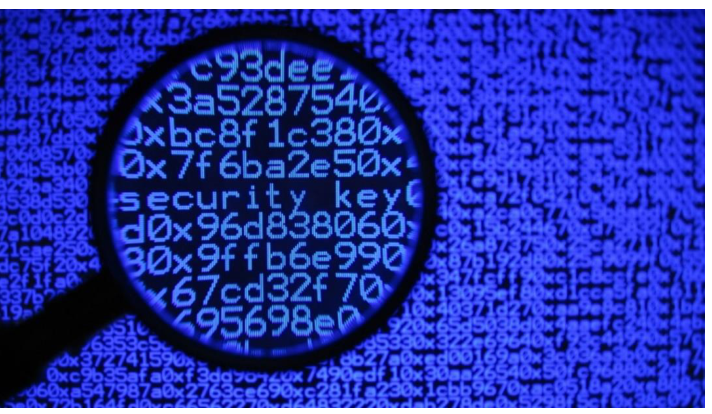
\includegraphics[width=77.91mm,height=114.05mm]{../../images/llm/page_011_img_01.png}%
\end{textblock*}

\end{document}
